\documentclass{article}%
\usepackage[T1]{fontenc}%
\usepackage[utf8]{inputenc}%
\usepackage{lmodern}%
\usepackage{textcomp}%
\usepackage{lastpage}%
\usepackage{authblk}%
\usepackage{graphicx}%
%
\title{Mutation of the Diamond{-}Blackfan Anemia Gene Rps7 in Mouse Results in Morphological and Neuroanatomical Phenotypes}%
\author{Christina Vega}%
\affil{CAS Key Laboratory of Pathogenic Microbiology and Immunology, Institute of Microbiology, Chinese Academy of Sciences, Beijing, China}%
\date{01{-}01{-}2012}%
%
\begin{document}%
\normalsize%
\maketitle%
\section{Abstract}%
\label{sec:Abstract}%
An article in the January/February 2012 issue of Cancer Cell reports that the effects of homogeneous peptide{-}protein interactions on expression of our cells circulating fat{-}derived par3 protein are similar to those found in non{-}fat secreted par3.\newline%
The newly reported results indicate that our cells can survive and reproduce with seemingly innocuous proteins. From the mid{-}eighth to the late nineteenth century, an understanding of what made or made dont makes our cells all different in every other way, said Michael Yu, Ph.D., professor of molecular and cell biology at Duke University Medical Center. And until now, no one really understood how our cells made different proteins in the way they did.\newline%
Tracking peptides from the early life of our cells to adulthood changes how our cells can be programmed to divide and reproduce. This gives us an unprecedented look at the first half of human evolution.\newline%
Until recently, finding peptides in cells has been mainly a matter of counting the number of eggs that hatched. But understanding how our cells produce proteins and incorporate more of them into their bodies could offer valuable clues to better understand the evolution of our own cancer cells.\newline%
Discovering the mechanisms at play in breast cancer cells really may hold the key to the uncontrolled growth and progression of tumors, Yu said.\newline%
He said that predicting how many eggs remain in cells isnt really that important. What is important, he said, is understanding the genes that make the cell look abnormal.\newline%
X{-}ray crystallography (X{-}ray C, or x{-}ray electron microscope)\newline%
Most cancer tumors look a lot like these {[}polyps{]}. So I thought we might be able to see how their cells grow and develop, Yu said.\newline%
Yu said researchers have identified a handful of small peptides (polyposis) that act as cellular predominates. They arent active in a whole lot of cells, but are integrated into a region of the cell that may make up their normal location.\newline%
But many of these polyposis look much less active than other phenotypes, Yu said.\newline%
To see if this observation can explain the biological effects of these peptides in breast cancer, researchers examined polyposis produced in a class of vertebrates, called MACH (microalbumin{-}iferos{-}oxygenase) cells. (The MACH cell is a type of pancreatic cancer cell that generally produces a low protein{-}density in a common tumor{-}derived protein.)\newline%
Those are cells that most likely produce good{-}quality protein, Yu said.\newline%
The finding, according to Yu, was a nice surprise.\newline%
The discovery is particularly important because this peptide profile has not been identified in other cell types, even inside parenteral and wound dressings, Yu said.\newline%
Yu, along with his fellow researchers from Duke and Harvard, traced the effectiveness of the peptides in targeting a protein called keratin (a protein that helps adhere to proteins.) They studied the peptides in a mouse model that had been genetically engineered to produce a low level of the protein.\newline%
By penetrating keratin, which is an established target of anticancer drugs, our laboratory tests revealed a severely diminished ability of the peptides to kill the keratin protein as well as a related biomarker, which is a cells bone{-}thinning protein kinase, Yu said.\newline%
He said that the idea is to design nanoparticles that could bind to keratin to kill it at its sites. That would provide the signature drug that will take the place of traditional therapies, such as anthracyclines, and thus be much more effective in preventing cancer cell development and the spread of cancer.

%
\subsection{Image Analysis}%
\label{subsec:ImageAnalysis}%


\begin{figure}[h!]%
\centering%
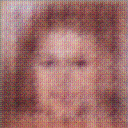
\includegraphics[width=150px]{500_fake_images/samples_5_475.png}%
\caption{A Man Wearing A Tie And A Hat}%
\end{figure}

%
\end{document}